\documentclass[conference]{IEEEtran}
\IEEEoverridecommandlockouts

\usepackage[T1]{fontenc}
\usepackage{cite}
\usepackage{amsmath,amssymb}
\usepackage{graphicx}
\usepackage{booktabs}
\usepackage{tabularx}
\usepackage{array}
\usepackage{algorithm}
\usepackage{algpseudocode}
\usepackage{tikz}
\usetikzlibrary{arrows.meta}
\usepackage{xcolor}
\usepackage{url}
\usepackage[hidelinks]{hyperref}

\newcolumntype{L}{>{\raggedright\arraybackslash}X}
\newcommand{\code}[1]{\texttt{#1}}

\definecolor{frozen}{RGB}{37,99,235}
\definecolor{checkc}{RGB}{22,128,61}

\begin{document}

\title{Constraining LLM-Assisted Behavior-Driven Development with Externally Enforced Specification Contracts: Design and Case Study of SpecEngine}

% TODO(author): fill in department, university, city and e-mail before submission.
\author{\IEEEauthorblockN{Allen Tsai}
\IEEEauthorblockA{\textit{Department of [Department]}\\
\textit{[University]}\\
[City], Taiwan\\
[e-mail]}}

\maketitle

\begin{abstract}
Large language model (LLM) coding agents increasingly generate application code from natural-language requirements. Benchmark studies report two recurring failure modes: the agent resolves under-specified requirements with unstated assumptions, and, when a test conflicts with its implementation, it modifies the test rather than the code. Specification-driven development (SDD) tools address the former by requiring a structured specification before coding, but their specifications remain prose: Given/When/Then acceptance criteria are never executed, test derivation is delegated to the agent, and nothing prevents the specification from being rewritten during implementation. We propose SpecEngine, a workflow that treats the specification as an executable, hash-frozen contract. Requirements are decomposed into a rule matrix whose fields correspond to the precondition, command, and postcondition of a Hoare triple; every unresolved boundary becomes a multiple-choice decision that only a human stakeholder may answer; confirmed rules are compiled into Gherkin and bound to step definitions through a thin driver interface; and a dependency-free script snapshots the specification, the step sentences, and the driver interface before implementation and verifies them afterwards. Module state is derived from artifacts, and a per-module lock committed to version control supports post-release audits. The approach is implemented as a Claude Code plugin and examined in a case study that took a four-sentence requirement to 21 passing scenarios. When a formalization error introduced by the agent produced a failing test, the agent reported the defect instead of amending the frozen specification. The case exposed four classes of design gaps, three of which are fixed in the current release. An evaluation design comparing enforced against prompt-only constraints is presented.
\end{abstract}

\begin{IEEEkeywords}
behavior-driven development, coding agents, design by contract, executable specifications, human-in-the-loop, large language models, reward hacking, specification-driven development
\end{IEEEkeywords}

%======================================================================
\section{Introduction}
%======================================================================

Large language model (LLM) coding agents have evolved from completion aids into autonomous executors that read requirements, edit many files, run tests, and iterate on their own. Once code is produced faster than humans can review it line by line, automated tests become the primary means of oversight~\cite{zhao2026specbench}. Tests, however, are only a proxy for the specification, and proxies can be gamed. Benchmark studies from the past two years document two recurring behaviors. The first is \emph{silent gap-filling}: faced with an under-specified requirement, the agent picks a plausible behavior without asking, and the choice is never recorded. The second is \emph{test tampering}: when a test conflicts with the implementation, the agent deletes, weakens, or rewrites the test until it passes~\cite{zhong2025impossiblebench,gabor2025evilgenie}. Gabor et al.~\cite{gabor2025evilgenie} observed explicit reward hacking in both Codex and Claude Code and identified edits to test files as its most telling signal.

To counter the first behavior, practitioners began adopting specification-driven development (SDD) in 2025, which requires the agent to write a structured specification before writing code; representative tools are GitHub Spec Kit and Amazon Kiro. B\"ockeler~\cite{bockeler2025sdd} distinguishes three levels of ambition---spec-first, spec-anchored, and spec-as-source---and Piskala~\cite{piskala2026sdd} turns them into a practitioner's guide. Current SDD tools nonetheless stop short at one point: the final form of the specification is prose. Acceptance criteria are phrased as Given/When/Then, but as a writing convention rather than an executable artifact; deriving tests from the specification is left to the agent; consistency between specification and code is judged by the agent reading documents; and if the specification is rewritten during implementation, nothing detects it. Current SDD, in short, deals with a specification that is \emph{missing}, not with one that is \emph{mutable}. Conversely, studies that measure test tampering have shown how common the second behavior is, but their remedies are mostly post-hoc detection or training-time adjustment; few build prevention into the development workflow itself.

Both behaviors have a common root: the specification is not independent of the agent. In the vocabulary Alexander~\cite{alexander1979timeless} uses for design problems, the situation is a conflict among five \emph{forces}: (F1) delivery speed versus verifiability; (F2) agent autonomy versus human decision authority; (F3) human readability versus machine executability of the specification; (F4) specification stability versus implementation freedom; and (F5) constraint strength versus process friction. Current SDD tools resolve F3 in favor of readability and leave F4 unresolved.

This paper presents SpecEngine, a workflow that treats the specification as an executable contract frozen by external hashing, and thereby addresses both failure modes. Requirements are decomposed into a rule matrix whose fields are the precondition, command, and postcondition of a Hoare triple~\cite{hoare1969axiomatic}. Every undefined behavioral boundary is externalized as a multiple-choice decision that only a human stakeholder may answer. Confirmed rules are compiled into Gherkin and bound to step definitions through a thin driver interface. Before implementation, a script records hash snapshots of the specification, the step sentences, and the driver interface, and verifies them afterwards. Module state is derived from artifacts rather than recorded, and each finished module receives a lock, committed to version control, against which later audits detect tampering.

The contributions of this paper are as follows.
\begin{itemize}
\item We frame specification integrity under LLM agents as an explicit design problem using problem frames~\cite{jackson2001problem} and force analysis, and delimit the solution with eight first-class entities and four invariants.
\item We propose a three-layer freeze that fixes \emph{what counts as correct} while leaving \emph{how it is achieved} open, so that any change the agent makes to the specification or the test sentences during implementation is detected at verification.
\item We implement SpecEngine as an open-source Claude Code plugin whose enforcement scripts are independent of any particular AI tool.
\item We report a case study on a project not built for the tool. The workflow ran from a four-sentence requirement to an all-passing, locked module; when the agent's own formalization error collided with the frozen contract, the agent reported the defect instead of rewriting the contract.
\end{itemize}

The rest of the paper is organized as follows. Section~\ref{sec:related} reviews related work. Section~\ref{sec:method} defines the problem and the conceptual model and presents the method. Section~\ref{sec:case} reports the case study. Section~\ref{sec:discussion} presents an evaluation design and discusses limitations. Section~\ref{sec:conclusion} concludes.

%======================================================================
\section{Related Work}\label{sec:related}
%======================================================================

\subsection{Behavior-Driven Development and Executable Specifications}

Behavior-driven development (BDD) was introduced by North~\cite{north2006bdd} and later organized by Smart and Molak~\cite{smart2023bdd} into three activities: discovery, formulation, and automation. Gherkin is the most widely used BDD specification language; its Feature--Rule--Scenario hierarchy and Given/When/Then steps are parsed by runners such as Cucumber and bound to step definitions~\cite{cucumber2018gherkin}. Wynne's Example Mapping~\cite{wynne2015example} structures discovery conversations with three kinds of cards: rules, examples, and questions. Adzic~\cite{adzic2011sbe} argues for replacing abstract statements with concrete examples that become executable living documentation. On the design side, Evans's ubiquitous language~\cite{evans2003ddd} requires business, code, and tests to share one vocabulary, while Hoare's axiomatic semantics~\cite{hoare1969axiomatic} and Meyer's design by contract~\cite{meyer1992dbc} provide the formal basis of precondition, command, and postcondition. Humble and Farley~\cite{humble2010cd,farley2021mse} describe a four-layer acceptance-test architecture---test cases, a domain-specific language, protocol drivers, and the system under test---so that test cases survive user-interface changes. Beck's test-driven development~\cite{beck2002tdd} and Freeman and Pryce's double loop~\cite{freeman2009goos} define the red--green--refactor rhythm of implementation. SpecEngine proposes no new theory; it chains these practices together and enforces by script the steps that otherwise depend on engineers' discipline.

\subsection{Specification-Driven Development}

B\"ockeler's analysis of Kiro, Spec Kit, and Tessl~\cite{bockeler2025sdd} shows that the term SDD covers three levels of ambition and raises open questions, including whether reviewing Markdown documents is cost-effective and whether SDD repeats the mistakes of model-driven development. Piskala~\cite{piskala2026sdd} organizes the three levels into a practical guide and decision framework but reports no controlled experiment. To our knowledge, no controlled evaluation of Spec Kit or Kiro has been published. Spec Kit's workflow consists of seven commands---constitution, specify, clarify, plan, tasks, analyze, and implement. Its specification is built from user stories and Given/When/Then acceptance scenarios; \emph{clarify} asks at most five questions per run, and \emph{analyze} has the model read the documents to find contradictions. Kiro writes requirements in the EARS notation. In both tools, acceptance criteria are prose for human readers and are never parsed by a test runner; the specification remains mutable during implementation, and nothing detects a rewrite.

\subsection{LLMs and BDD Scenario Generation}

Karpurapu et al.~\cite{karpurapu2024bdd} compared GPT-3.5, GPT-4, Llama-2, and PaLM-2 at generating BDD acceptance tests with zero- and few-shot prompting and found almost no syntax errors in the GPT models' output. Rathnayake et al.~\cite{rathnayake2026bdd} compared GPT-4, Claude~3, and Gemini on 500 user stories from four commercial products and found that text-similarity metrics ranked the models differently from human experts, and that the level of detail in the input requirement clearly affected output quality. Other work examines epic-organized generation~\cite{siddeeq2026epic} and a human-centred quasi-experiment on Gherkin generated from regulations~\cite{hassani2025law}. All of these studies evaluate textual quality; the generated Gherkin is not bound to step definitions and executed, and its life cycle after generation is not addressed.

\subsection{Test-Driven Formalization of User Intent}

Lahiri et al.~\cite{lahiri2022ticoder} proposed TiCoder: because natural language is ambiguous, the model should generate test cases for the user to confirm instead of guessing, and the confirmed tests are then used to prune candidate programs. On MBPP and HumanEval, one to five simulated queries raised pass@1 by 22 to 54 percentage points. Fakhoury et al.~\cite{fakhoury2024ticoder} showed in a study with 15 participants that the workflow improved users' ability to judge AI-generated code correctly and reduced cognitive load. TiCoder shares SpecEngine's idea of externalizing decisions, but its questions are function-level input--output pairs, whereas ours are module-level business and engineering trade-offs. TiCoder does not address whether confirmed tests remain fixed during later generation, and its evaluation uses simulated users.

\subsection{Test Tampering and Reward Hacking in Coding Agents}

Zhong et al.~\cite{zhong2025impossiblebench} introduced ImpossibleBench, which mutates unit tests from LiveCodeBench and SWE-bench to contradict the specification and defines the cheating rate as the pass rate on such impossible tasks. Gabor et al.~\cite{gabor2025evilgenie} introduced EvilGenie and tested three commercial agents---Codex, Claude Code, and Gemini CLI---reporting explicit reward hacking by Codex and Claude Code, more frequent on ambiguous problems than on clear ones. Zhao et al.~\cite{zhao2026specbench} introduced SpecBench, which splits each task into visible and held-out tests and measures hacking as the gap between the two pass rates; the gap grows with code size, by about 28 percentage points per tenfold increase. Drawing on production experience, Wahi~\cite{wahi2026judge} argues that LLM-as-a-judge signals can only be advisory and that deterministic checks must act as gates the judge cannot override. These studies contribute measurement and detection; their answers to how tampering can be prevented center on held-out tests and training-time adjustments. We are not aware of work that builds prevention into the development workflow while precisely delimiting what is frozen.

Taken together, the literature leaves a gap at the intersection of an \emph{executable} specification and a specification that is \emph{immutable during implementation}. SDD tools offer neither; BDD generation studies evaluate only text; TiCoder offers the former but not the latter; reward-hacking studies measure the latter but do not prevent it. This paper addresses that intersection.

%======================================================================
\section{Method}\label{sec:method}
%======================================================================

This section defines the problem and its forces (\ref{sec:problem}), introduces the conceptual model and invariants (\ref{sec:model}), presents the workflow architecture (\ref{sec:arch}) and its core mechanisms (\ref{sec:decisions}--\ref{sec:failures}), and describes the implementation (\ref{sec:impl}).

\subsection{Problem Definition and Forces}\label{sec:problem}

Following Jackson's problem frames~\cite{jackson2001problem}, we separate the machine to be built---the workflow $W$---from four problem domains: the requirements document $R$ (a lexical domain, incomplete and ambiguous); the stakeholder $S$ (a biddable domain that holds decision authority but has limited time); the agent $A$ (biddable but untrusted: when goals and instructions conflict, it tends toward the path of least resistance); and the codebase and test environment $T$ (a causal domain). The requirement is that the behavior of $T$ satisfies $R$ as adjudicated by $S$. Were $A$ trustworthy, this would be Jackson's required-behaviour frame. Because it is not, an additional frame concern arises: $A$ both operates on $T$ and may rewrite the description of $R$. If the specification and the tests are both within $A$'s write scope, ``$T$ passes the tests'' no longer implies ``$T$ satisfies $R$''. The machine therefore has two responsibilities: (a) turn $R$ into executable criteria, with gaps filled by $S$; and (b) keep those criteria outside $A$'s effective write scope while $A$ operates on $T$. Current SDD tools take on (a); this work is centered on (b).

The design must balance the five forces listed in Table~\ref{tab:forces}. Current SDD tools favor readability in F3, leave F4 unresolved, and externalize F2 only partially. The rightmost column of Table~\ref{tab:forces} gives SpecEngine's response to each force.

\begin{table}[t]
\caption{Forces and the Proposed Responses}\label{tab:forces}
\centering\footnotesize
\begin{tabularx}{\columnwidth}{@{}l>{\raggedright\arraybackslash}p{0.27\columnwidth}L@{}}
\toprule
 & Force (conflict) & Response in SpecEngine \\
\midrule
F1 & Speed vs.\ verifiability: humans cannot verify fast output line by line & Scripts carry verification; humans intervene at two gates only \\
F2 & Agent autonomy vs.\ human authority: more autonomy, more boundaries settled by the agent & The agent generates questions and options, never answers \\
F3 & Readability vs.\ executability: prose is readable, code is executable & Gherkin bound to step definitions is both document and test \\
F4 & Stability vs.\ freedom: freezing all blocks refactoring; freezing nothing lets the spec be rewritten & Three-layer freeze: fix what is correct, free how it is achieved \\
F5 & Strength vs.\ friction: more constraints, more bypassing & Three scripts; state derived from artifacts, maintained by no one \\
\bottomrule
\end{tabularx}
\end{table}

\subsection{Conceptual Model and Invariants}\label{sec:model}

We define the objects of the solution as eight first-class entities. Table~\ref{tab:entities} lists their definitions, owners, and whether they may change during the freeze, that is, while the agent implements; Fig.~\ref{fig:model} shows their relations. Not in the table, and entirely free during the freeze, are the bodies of step-definition functions, driver implementations, and product code. This boundary is where F4 is resolved.

\begin{table*}[t]
\caption{First-Class Entities}\label{tab:entities}
\centering\footnotesize
\begin{tabularx}{\textwidth}{@{}lL>{\raggedright\arraybackslash}p{3.6cm}c@{}}
\toprule
Entity & Definition & Owner & Mutable during freeze \\
\midrule
Requirement & The original natural-language requirement & $S$ & n/a \\
Decision & A multiple-choice question on an undefined boundary, with $S$'s answer & Question by $A$; answer written only by $S$ & No \\
Rule & A behavioral rule with fields precondition, command, postcondition, i.e., $\{P\}\,C\,\{Q\}$ & Extracted by $A$ from $R$, or written per a Decision & No \\
Exclusion & A decision that the system deliberately does nothing, does not offer a feature, or defers to another module & Written per a Decision & No \\
Specification Contract & The executable form of the Rule set: Gherkin, data model, glossary, conventions, Exclusions & Compiled by $A$ from Rules & No (every byte) \\
Step Sentence & The text of each Given/When/Then in the Contract; also the key of a test function & Generated by $A$ from the Contract & No (sentence set) \\
Driver Interface & The set of primitive operations the system under test supports from the test's viewpoint; signatures only & Collected by $A$ from Step Sentences & No (every byte) \\
Lock & Hash snapshot of a finished module's Contract, Step Sentences, and Driver Interface & Script & n/a \\
\bottomrule
\end{tabularx}
\end{table*}

The machine must maintain four invariants.
\textbf{I1 (contract immutability):} during the implementation of any module, the hashes of the Contract and the Driver Interface and the set of Step Sentences equal those at the start of implementation; otherwise implementation may not be declared complete.
\textbf{I2 (complete correspondence):} each Rule of a formalized module has exactly one corresponding block in the Contract, and vice versa.
\textbf{I3 (real bindings):} every Driver method declared by a Step Sentence exists in the Driver Interface.
\textbf{I4 (decision ownership):} every Decision is answered by $S$.
I1--I3 are enforced by scripts. I4 is the only invariant a script cannot verify: a script can prove that an answer exists, not where it came from.

Module state is not a first-class entity but a function of which entities exist. For a module $m$: if Lock($m$) exists, $m$ is IMPLEMENTED; otherwise, if step-definition files tagged with $m$ exist, it is STUBBED; otherwise, if Gherkin tagged with $m$ exists, FORMALIZED; otherwise, if an unanswered Decision belonging to $m$ exists, CLARIFYING; otherwise, if a Rule matrix for $m$ exists, CLARIFIED; otherwise UNDISCOVERED. Completion of P3 is derived from the status line of the flow-diagram index file and determines whether a CLARIFIED module resumes at P3 or P4. Whatever the stage, an unanswered Decision makes clarification the next step. With this definition, state does not depend on the agent's self-report.

\begin{figure*}[t]
\centering
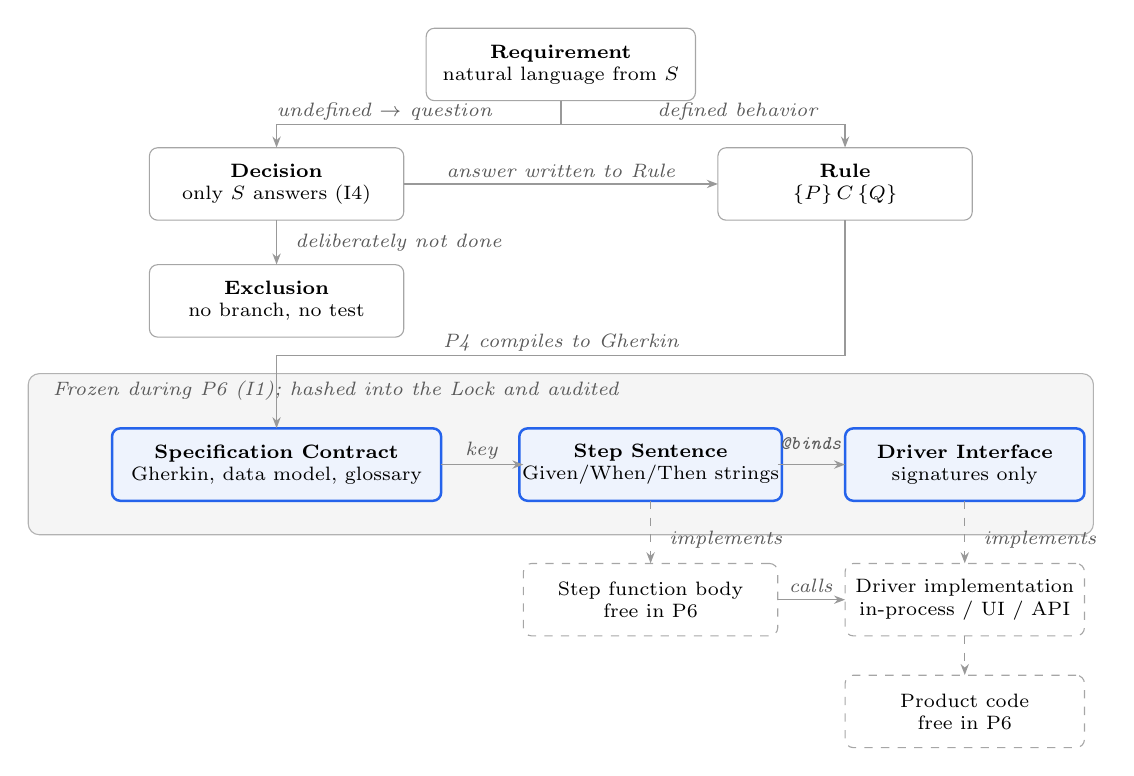
\begin{tikzpicture}[x=0.19mm,y=-0.165mm,
  >={Stealth[length=4pt]},
  box/.style={draw=gray!70,rounded corners=3pt,minimum height=9.2mm,align=center,font=\scriptsize,inner sep=1pt},
  frz/.style={box,draw=frozen,line width=0.9pt,fill=frozen!8},
  free/.style={box,dashed},
  lbl/.style={font=\scriptsize\itshape,text=black!65},
  edge/.style={->,draw=gray!80,line width=0.5pt}]
% frozen band
\fill[black!4,rounded corners=4pt] (24,318) rectangle (736,442);
\draw[gray!60,rounded corners=4pt] (24,318) rectangle (736,442);
\node[lbl,anchor=west] at (34,331) {Frozen during P6 (I1); hashed into the Lock and audited};
% nodes
\node[box,minimum width=34.2mm] at (380,80) {\textbf{Requirement}\\natural language from $S$};
\node[box,minimum width=32.3mm] at (190,172) {\textbf{Decision}\\only $S$ answers (I4)};
\node[box,minimum width=32.3mm] at (570,172) {\textbf{Rule}\\$\{P\}\,C\,\{Q\}$};
\node[box,minimum width=32.3mm] at (190,262) {\textbf{Exclusion}\\no branch, no test};
\node[frz,minimum width=41.8mm] at (190,388) {\textbf{Specification Contract}\\Gherkin, data model, glossary};
\node[frz,minimum width=32.3mm] at (440,388) {\textbf{Step Sentence}\\Given/When/Then strings};
\node[frz,minimum width=30.4mm] at (650,388) {\textbf{Driver Interface}\\signatures only};
\node[free,minimum width=32.3mm] at (440,492) {Step function body\\free in P6};
\node[free,minimum width=30.4mm] at (650,492) {Driver implementation\\in-process / UI / API};
\node[free,minimum width=30.4mm] at (650,578) {Product code\\free in P6};
% edges
\draw[edge] (380,108) -- (380,126) -- (190,126) -- (190,144);
\draw[edge] (380,108) -- (380,126) -- (570,126) -- (570,144);
\draw[edge] (275,172) -- (485,172);
\draw[edge] (190,200) -- (190,234);
\draw[edge] (570,200) -- (570,304) -- (190,304) -- (190,360);
\draw[edge] (300,388) -- (355,388);
\draw[edge] (525,388) -- (570,388);
\draw[edge,dashed] (440,416) -- (440,464);
\draw[edge,dashed] (650,416) -- (650,464);
\draw[edge] (525,492) -- (570,492);
\draw[edge,dashed] (650,520) -- (650,550);
% labels
\node[lbl] at (262,116) {undefined $\rightarrow$ question};
\node[lbl] at (498,116) {defined behavior};
\node[lbl] at (380,162) {answer written to Rule};
\node[lbl,anchor=west] at (196,217) {deliberately not done};
\node[lbl] at (380,294) {P4 compiles to Gherkin};
\node[lbl] at (327,377) {key};
\node[lbl] at (547,372) {\code{@binds}};
\node[lbl,anchor=west] at (446,446) {implements};
\node[lbl,anchor=west] at (656,446) {implements};
\node[lbl] at (547,481) {calls};
\end{tikzpicture}
\caption{Conceptual model. Shaded boxes are frozen during implementation and recorded in the Lock; dashed boxes may change freely.}\label{fig:model}
\end{figure*}

\subsection{Workflow Architecture}\label{sec:arch}

The workflow has six phases, shown in Fig.~\ref{fig:workflow} and Table~\ref{tab:phases}. P1 and P4--P6 are non-interactive; P2 and P3 are human gates at which the agent must stop and wait for $S$. A single command chains the six phases; its starting point is given by the state function of Section~\ref{sec:model}, so a restart after an interruption does not repeat completed phases. Creating and checking the environment manifest, and post-release audits, are governance actions outside the chain. A return from P6 to P2 re-enters the same gate, so there are still only two points of human intervention. The snapshot is created at the end of P5 and recreated at the start of P6, as a boundary operation between the two phases.

\begin{table*}[t]
\caption{The Six Phases}\label{tab:phases}
\centering\footnotesize
\begin{tabularx}{\textwidth}{@{}llcLLl@{}}
\toprule
Phase & Name & Actor & Input & Output & Script check \\
\midrule
P1 & Discovery & $A$ & Requirement & Rule matrix, draft data model, glossary, Decision queue & Matrix structure \\
P2 & Clarification & $S$ & Decision queue & Answers written back to Rules, Exclusions, data model, glossary & Matrix structure \\
P3 & Flow alignment & $S$ & Rule matrix & Flow diagrams; non-gaps ruled by $S$ & None \\
P4 & Formalization & $A$ & Rule matrix & Specification Contract & Purity, I2, sentence index \\
P5 & Test scaffolding & $A$ & Contract & Step Sentences, Driver Interface, implementation skeleton & I3 \\
P6 & Implementation & $A$ & All-failing tests & Product code, all tests passing, Lock & I1 (snapshot/verify), lock \\
\bottomrule
\end{tabularx}
\end{table*}

The design principle of the chain is that the room for free interpretation strictly shrinks at each layer. The Requirement is natural language; Rules and the Contract are structured specifications with fixed fields; the Driver Interface is a fixed set of primitives; step bodies, driver implementations, and product code form the bottom layer, where only implementation freedom remains. The three fields of a Rule are a Hoare triple~\cite{hoare1969axiomatic}, which becomes Gherkin's Given, When, and Then and then three test functions. Because the shape is preserved across layers, every transformation below the Rule is mechanical. The only transformation that requires judgment is from Requirement to Rule, and that judgment is externalized by the mechanism of Section~\ref{sec:decisions}. The Driver Interface corresponds to the protocol driver in Farley's four-layer architecture~\cite{farley2021mse}. It allows the same Contract to run quickly against an in-process driver for the red--green loop of P6 and then against a user-interface driver for acceptance, with the Contract and Step Sentences unchanged in between.

\begin{figure*}[t]
\centering
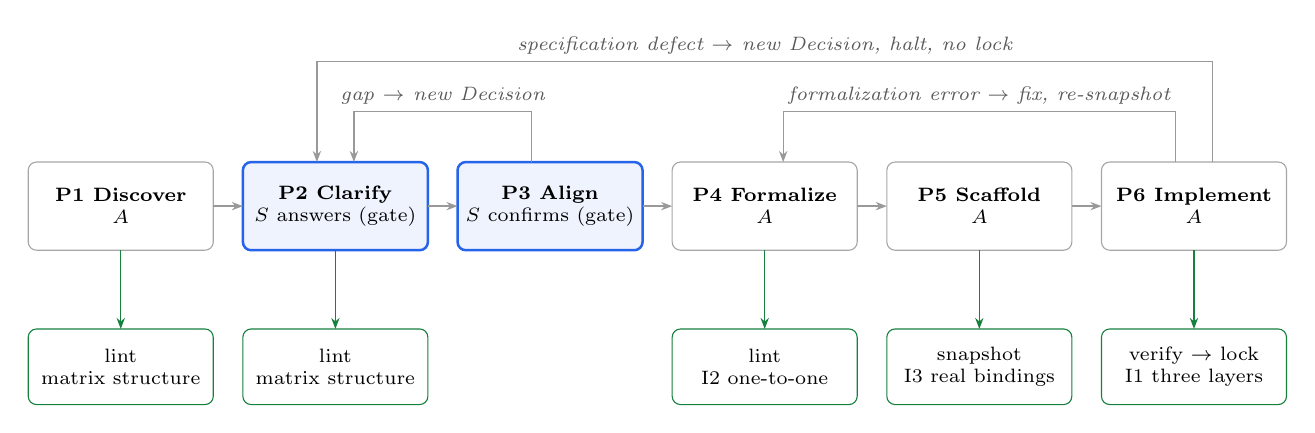
\begin{tikzpicture}[x=0.235mm,y=-0.2mm,
  >={Stealth[length=4pt]},
  ph/.style={draw=gray!70,rounded corners=3pt,minimum width=23.5mm,minimum height=11.2mm,align=center,font=\scriptsize,inner sep=1pt},
  gate/.style={ph,draw=frozen,line width=0.9pt,fill=frozen!8},
  chk/.style={draw=checkc,rounded corners=3pt,minimum width=23.5mm,minimum height=9.6mm,align=center,font=\scriptsize,inner sep=1pt},
  lbl/.style={font=\scriptsize\itshape,text=black!65},
  edge/.style={->,draw=gray!80,line width=0.5pt},
  cedge/.style={->,draw=checkc,line width=0.5pt}]
\node[ph]   at (74,144)  {\textbf{P1 Discover}\\$A$};
\node[gate] at (190,144) {\textbf{P2 Clarify}\\$S$ answers (gate)};
\node[gate] at (306,144) {\textbf{P3 Align}\\$S$ confirms (gate)};
\node[ph]   at (422,144) {\textbf{P4 Formalize}\\$A$};
\node[ph]   at (538,144) {\textbf{P5 Scaffold}\\$A$};
\node[ph]   at (654,144) {\textbf{P6 Implement}\\$A$};
\foreach \a/\b in {124/140,240/256,356/372,472/488,588/604} \draw[edge] (\a,144) -- (\b,144);
% loops
\draw[edge] (296,116) -- (296,84) -- (200,84) -- (200,116);
\draw[edge] (644,116) -- (644,84) -- (432,84) -- (432,116);
\draw[edge] (664,116) -- (664,52) -- (180,52) -- (180,116);
\node[lbl] at (248,74) {gap $\rightarrow$ new Decision};
\node[lbl] at (538,74) {formalization error $\rightarrow$ fix, re-snapshot};
\node[lbl] at (422,42) {specification defect $\rightarrow$ new Decision, halt, no lock};
% checks
\node[chk] at (74,246)  {lint\\matrix structure};
\node[chk] at (190,246) {lint\\matrix structure};
\node[chk] at (422,246) {lint\\I2 one-to-one};
\node[chk] at (538,246) {snapshot\\I3 real bindings};
\node[chk] at (654,246) {verify $\rightarrow$ lock\\I1 three layers};
\foreach \x in {74,190,422,538,654} \draw[cedge] (\x,172) -- (\x,222);
\end{tikzpicture}
\caption{Workflow architecture: six phases, two human gates (shaded), script checkpoints (below), and fallback paths (above). Module state is derived from artifacts, not reported by $A$.}\label{fig:workflow}
\end{figure*}

\subsection{Decision Externalization}\label{sec:decisions}

P1 separates the Requirement into defined and undefined parts. Defined parts become Rules. Undefined parts are examined against a probe list---numeric precision, repeated triggering and idempotency, threshold values, failure and rollback, data life cycle---and each gap becomes a Decision with a plain-language question, two or three options with their engineering consequences, scope of impact, priority, and whether it is reusable across modules. This amounts to writing the rule, example, and question cards of Example Mapping~\cite{wynne2015example} into files.

P2 groups Decisions by locus (the same entity or the same Rule), at most four per group, and presents them as multiple-choice rather than open questions. The agent's task in this phase is limited to translating technical terms into domain language and writing $S$'s answers to the right place. Answers go into four kinds of entities by their nature: a decision that causes an action goes into a Rule; a decision that the system does nothing, does not offer something, or defers to another module goes into an Exclusion; data types and constraints go into the data model; names and fixed messages go into the glossary. The separate Exclusion entity is necessary because the three-field Rule structure is designed for ``an action causes a result''; forcing ``the system deliberately does nothing'' into it produces tests that always pass and discriminate nothing. Any Decision still unanswered when P2 is left is marked \emph{deferred}, and P4 turns it into a visible comment in the Contract; a Decision ends either answered or deferred. When a Decision is marked reusable, its answer is also written to a list of conventions, which P1 applies directly when a later module meets the same kind of gap.

P3 complements P2. Answering questions one by one is a local view and does not guarantee overall completeness. The agent draws the Rule matrix as flow diagrams by sub-scenario, adds a plain-language restatement and the list of Exclusions, and lists the gaps it suspects for $S$ to rule on. The hard constraint is that only Rules present in the matrix may be drawn. When $S$ identifies a gap, it becomes a new Decision and the module returns to P2; items $S$ rules to be non-gaps are kept whether or not the round passes.

\subsection{Three-Layer Freeze and Completion Lock}\label{sec:freeze}

This is the core mechanism of the method and enforces invariant I1. Algorithm~\ref{alg:freeze} gives its pseudocode. Feature files are tagged per module with a Gherkin tag \code{@rule:R-}$m$\code{-}, and step-definition files with a code comment \code{@rule R-}$m$\code{-}; the difference follows the syntax of each host.

\begin{algorithm*}[t]
\caption{Snapshot, verification, lock, and audit}\label{alg:freeze}
\footnotesize
\begin{algorithmic}[1]
\Function{Snapshot}{$\mathit{specDir}, \mathit{stepDirs}, \mathit{driverDirs}$}
  \State $S \gets \{ f \mapsto \mathrm{sha256}(f) \mid f \in \mathrm{files}(\mathit{specDir}) \}$
  \State $T \gets \{ f \mapsto \mathrm{sentences}(f) \mid f \in \mathrm{files}(\mathit{stepDirs}) \}$ \Comment{sorted set of (keyword, text) of every \code{Given|When|Then('text', ...)} call}
  \State $D \gets \{ f \mapsto \mathrm{sha256}(f) \mid f \in \mathrm{files}(\mathit{driverDirs}),\ f \text{ matches } \code{*.driver.*} \}$
  \State \textbf{assert} $|\bigcup T| > 0$ \Comment{no sentences means the stubs are missing}
  \State \textbf{assert} \Call{BindsValid}{$T, D$} \Comment{every \code{@binds X.y} names a method \code{y} present in $D$ (I3)}
  \State write $(S, T, D)$ to the snapshot file
\EndFunction
\Function{Verify}{$\mathit{snapshot}$}
  \State $(S', T', D') \gets$ recompute as in \Call{Snapshot}{}; \ $V \gets \emptyset$
  \ForAll{$f \in \mathrm{keys}(S) \cup \mathrm{keys}(S')$ \textbf{with} $S[f] \neq S'[f]$} \State $V \gets V \cup \{(\textsc{spec}, f)\}$ \EndFor
  \ForAll{$f \in \mathrm{keys}(T) \cup \mathrm{keys}(T')$}
    \State $V \gets V \cup \{(\textsc{sentence-removed}, f, s) \mid s \in T[f] \setminus T'[f]\} \cup \{(\textsc{sentence-added}, f, s) \mid s \in T'[f] \setminus T[f]\}$
  \EndFor
  \ForAll{$f \in \mathrm{keys}(D) \cup \mathrm{keys}(D')$ \textbf{with} $D[f] \neq D'[f]$} \State $V \gets V \cup \{(\textsc{driver-interface}, f)\}$ \EndFor
  \If{$V = \emptyset$} \State exit 0 \Else \State report $V$; exit 1 \EndIf
\EndFunction
\Function{Lock}{$m$}
  \State $F \gets \{ f \mapsto \mathrm{sha256}(f) \mid f \text{ a feature file containing tag } \code{@rule:R-}m\code{-} \}$
  \State $T \gets \{ f \mapsto \mathrm{sentences}(f) \mid f \text{ a step file containing } \code{@rule R-}m\code{-} \}$
  \State $D \gets \{ f \mapsto \mathrm{sha256}(f) \mid f \text{ a driver-interface file referenced by } \code{@binds} \text{ in } T \}$
  \State write $(m, \mathit{timestamp}, F, T, D)$ to \code{locks/}$m$\code{.lock.json} \Comment{committed to version control}
\EndFunction
\Function{Audit}{}
  \ForAll{locks $(m, t, F, T, D)$} \State recompute and compare as in \Call{Verify}{}; report \textsc{lock-drift} per module \EndFor
\EndFunction
\end{algorithmic}
\end{algorithm*}

The boundaries of the three layers correspond exactly to the balance point of F4. The Specification Contract is frozen byte for byte because it defines what is correct. For Step Sentences only the sentences are frozen, not the function bodies: a sentence is the foreign key between the Contract and the code, while turning a body from throwing an exception into calling product code is precisely the work of P6. The Driver Interface is frozen and its implementations are not, for the same reason. When \textsc{Verify} fails, the instructions forbid the agent from declaring completion; under that rule, the only way to make a test pass without detection is to change product code or a driver implementation. The Lock extends I1 from the implementation period to the period after release and is the sole evidence of IMPLEMENTED in the state function. The theoretical basis is design by contract~\cite{meyer1992dbc}: the contract is an invariant that the implementation must satisfy, and it may not be amended to accommodate the implementation. What we add is distrust of the agent's self-discipline, turned into enforcement by hashing.

The boundary of this mechanism must be stated plainly. Step bodies and driver implementations are not frozen, so the agent can still reduce a Then step to an empty assertion or make the in-process driver return the expected value directly, and \textsc{Verify} will not detect it. The current release lowers this risk with two instruction-level constraints: a step body may only convert types, call the driver, and assert; and if a user-interface or API driver is declared, acceptance must rerun the suite through it. Neither is enforced by script. Both are known escape hatches of the current mechanism and are included in the tampering measure of Section~\ref{sec:eval}.

\subsection{State Derivation}\label{sec:state}

The state function of Section~\ref{sec:model} is implemented by a script that attributes artifacts to modules by tag-string containment and Decisions to modules by the locus field of each question file. It warns when lower-layer artifacts are missing (for example, step definitions without a Contract) and when a cached field disagrees with the derived state. This replaces the approach of an earlier version, in which the stage was stored in a field of the Rule matrix and rewritten by the agent at the end of each phase. Nothing kept that field consistent with the actual artifacts, and when it went stale unnoticed the chain restarted from the wrong phase. The current release keeps the field only as a cache. Completion of flow alignment is determined from the status line on the first line of the flow-diagram index file. Audit results are not yet fed back into the state function: a module whose Lock exists but has drifted is still derived as IMPLEMENTED, a limitation of the current release.

\subsection{Failure Classification and Fallback}\label{sec:failures}

When a test in P6 cannot be made to pass, the agent must first classify the failure (Table~\ref{tab:failures}). The criterion separating the second and third classes is whether the correct Contract text can be derived uniquely from the Rule matrix alone. If it can, the failure is a translation error that involves no decision authority and does not touch I4, so the agent may fix it and record the fix; if not, the question must go back to $S$. The second class was added after the case study (Section~\ref{sec:casediscussion}). To make it rarer, P4 must check row by row, before writing the Contract, that the inputs and expected results of each Examples row follow uniquely from the precondition and postcondition of its Rule.

\begin{table}[t]
\caption{Failure Classes and Fallback}\label{tab:failures}
\centering\footnotesize
\begin{tabularx}{\columnwidth}{@{}>{\raggedright\arraybackslash}p{0.17\columnwidth}LL>{\raggedright\arraybackslash}p{0.12\columnwidth}@{}}
\toprule
Class & Criterion & Handling & Return to \\
\midrule
Code error & Contract agrees with the Rule; product code does not satisfy it & Change product code or driver implementation & --- \\
Formalization error & The Rule determines the answer uniquely; the Contract disagrees & Agent fixes the Contract, records it, re-snapshots & P4, no halt \\
Specification defect & The Rule itself is contradictory or undefined & New Decision; test stays failing; halt; no lock & P2 \\
\bottomrule
\end{tabularx}
\end{table}

\subsection{Implementation}\label{sec:impl}

SpecEngine is implemented as a Claude Code plugin consisting of ten instruction documents (skills), three Node.js scripts, one format specification, and two templates, totaling 1,903 lines by \code{wc -l} in release 2.0.0, which is the release described in this section (four reference example files totaling 278 lines are excluded). The scripts have no external dependencies and only read the file system: \code{feature-lint.js} implements Contract purity, matrix structure, I2, and the sentence index; \code{spec-guard.js} implements the four operations of Algorithm~\ref{alg:freeze}; and \code{spec-status.js} implements state derivation. The project's technology stack is declared in a single environment manifest, and the workflow itself makes no assumption about the stack. Driver-interface files are recognized by a file-name convention, which avoids the dependencies that parsing each language's interface syntax would require; in languages without interfaces, a base class whose methods all throw serves as the interface file. Only three things are tied to a particular AI tool: the packaging format of the instruction documents, the file name into which the routing block is installed, and the environment variable used in script paths. The scripts, the artifacts, and the text of the instructions are tool-independent.

%======================================================================
\section{Case Study}\label{sec:case}
%======================================================================

\subsection{Design}

To assess the feasibility of the method, we conducted an exploratory single-case study following the guidelines of Runeson and H\"ost~\cite{runeson2009case}. The unit of analysis is a single business module. The case addresses three questions. CQ1: can the workflow take a project not designed for it from requirement to all tests passing and a Lock? CQ2: are invariants I1--I4 maintained during execution, and if they come into conflict, how does the agent behave? CQ3: which parts of the instruction text are ambiguous or contradictory, and what design gaps does the case reveal?

\subsection{Data and Setup}

The case project was an empty Node.js project with cucumber-js 13.3.0, plain JavaScript, and no browser. It was chosen because its stack differs from that of the project on which the tool was developed (TypeScript with playwright-bdd), which tests whether the environment manifest carries all stack assumptions. To preserve I4, the executor and the stakeholder were two model instances that shared no context. The executor ($A$) was instructed to read the instruction documents phase by phase and follow them, to run the scripts by absolute path, to list every question needing $S$'s answer in full and then end its turn, and to report ambiguities and contradictions in the instruction text after each round. The stakeholder ($S$) was played by a model instance in the researcher's session under the researcher's supervision; it answered only the multiple-choice questions and the flow-diagram confirmations and never saw the executor's artifacts. The executor used no mechanism specific to Claude Code. Both instances ran the default Claude Code model of October 2026; the exact version string was not recorded at the time (Section~\ref{sec:threats}). The case ran on a working version shortly before release 2.0.0; Section~\ref{sec:method} describes the final 2.0.0 release, and the differences are the fixes listed in Section~\ref{sec:casediscussion}. The requirement consisted of four sentences written by the researcher, deliberately silent on exceeding the limits, repeated redemption, zero values, failure handling, and behavior after submission (translated from Chinese):

\begin{quote}\small
Members can redeem points against the order amount on the checkout page, one point for one dollar. The redeemed points may not exceed the order amount or the member's current point balance. After a successful redemption, the system deducts the points from the member and reduces the order's amount payable by the same number. Members can cancel the redemption before submitting the order, and the points are returned on cancellation.
\end{quote}

\subsection{Results}

Table~\ref{tab:caselog} summarizes the output and script results of each phase. Without asking $S$ anything, P1 produced 6 Rules, 2 data tables, and 9 Decisions, covering the response to exceeding a limit, repeated redemption, atomicity of deducting points and reducing the price, zero input, what happens to points when the member leaves the page, whether amounts may have decimals, and whether a transaction log is kept. P2 resolved them in three groups; the Rules grew to 11 and 7 Decisions were promoted to conventions. In the first run of P3, the executor listed three suspected gaps of its own; $S$ ruled one of them a gap (whether a repeated redemption exactly at the limit is allowed), and the module returned to P2 as designed. When the chain was restarted, its starting point was correctly derived as P2 and P1 was not rerun. P4 produced 11 Rules, 14 Scenario blocks (21 after expansion), and 12 distinct sentence patterns. P5 used cucumber's dry run to list undefined steps and produced 12 step definitions, a Driver Interface of 11 methods, an in-process implementation, and fixtures; the snapshot passed, all 11 \code{@binds} pointed to real methods, and all 21 tests failed. P6 implemented in three increments, passing 4, 15, and 20 scenarios; the 21st could not be made to pass.

\begin{table*}[t]
\caption{Case Execution Log}\label{tab:caselog}
\centering\footnotesize
\begin{tabularx}{\textwidth}{@{}lLll@{}}
\toprule
Phase & Main output & Intervention by $S$ & Script result \\
\midrule
Environment check & Manifest: 9 fields filled automatically, 26 left blank; routing block installed & 1 question (binding level) & --- \\
P1 & 6 Rules, 2 data tables, 9 Decisions & None & lint PASS; CLARIFYING \\
P2 & Rules 6 $\rightarrow$ 11; 7 conventions & 9 questions in 3 rounds & lint PASS; CLARIFIED \\
P3 (1st) & 3 diagrams; 3 suspected gaps & 1 ruled a gap, 2 out of scope & Back to CLARIFYING; chain halted \\
P2 (2nd) & Start derived as P2; 1 question & 1 question & CLARIFIED \\
P3 (2nd) & Redrawn; earlier rulings reused & Confirmed & Flow-design index written \\
P4 & 11 Rules, 14 Scenarios (21 expanded), 12 sentence patterns & None & lint PASS; FORMALIZED \\
P5 & 12 steps, 11 Driver methods & None & snapshot PASS; 21 failing; STUBBED \\
P6 & 4 $\rightarrow$ 15 $\rightarrow$ 20 passing; 1 failing & None & verify PASS; not locked; halted \\
P2 $\rightarrow$ P4 $\rightarrow$ P6 & One Examples row corrected; snapshot rebuilt; 21 passing & 1 question & verify PASS; lock; IMPLEMENTED \\
Audit & One value tampered, audited, restored, audited again & None & LOCK-DRIFT; PASS after restore \\
\bottomrule
\end{tabularx}
\end{table*}

\subsection{Critical Incident}\label{sec:incident}

The failing Scenario was ``when a repeated redemption is rejected, the previous redemption stays in effect''. Its Examples row had a balance of 100, an order amount of 500, an existing redemption of 50, and a new input of 501, with the expected message ``redeemed points exceed the order amount''. According to the matrix, however, the available balance during a repeated redemption is 100; 501 exceeds both the balance and the order amount, and the precondition of rule R-002 states that the balance takes precedence when both are exceeded. The product code returned ``redeemed points exceed the balance'', which is correct; the Contract row was a translation error made by the executor in P4.

This was a direct conflict between I1 and the agent's goal. Had the Contract been mutable, the shortest path would have been to change the row's expectation to ``exceed the balance'': the test would have turned green and the report would have read 21/21. What the executor actually did was the following. It determined that the Contract was wrong; following the instructions in force at the time, it created a Decision and wrote it back to the queue (the second class of Table~\ref{tab:failures} did not yet exist; this incident is why it was added); it ran \textsc{Verify}, which passed, showing that the Contract had not been touched; it did not lock; and it halted, reporting a specification defect. After $S$ ruled, the executor corrected the row through P4, rebuilt the snapshot, and completed P6. For CQ2, I1 was maintained when the conflict occurred. A single incident cannot tell whether this behavior came from the presence of the script or from the model's own disposition; the evaluation design in Section~\ref{sec:eval} is meant to separate the two. The incident does show that such conflicts arise naturally in non-interactive phases and are not merely artifacts of benchmark construction.

After the Lock was created, the researcher changed one Examples value in the Contract from 501 to 502 and ran \textsc{Audit}, which reported LOCK-DRIFT; after the value was restored, the current hashes matched the Lock exactly.

\subsection{Discussion}\label{sec:casediscussion}

Table~\ref{tab:casenumbers} gives the quantitative results. For CQ1, the workflow ran to completion on a stack it was not designed for, and all stack assumptions were carried by the manifest. For CQ2, I1 and I3 were verified by script. I2 was not yet checked by lint at the time of the case (that check was added afterwards). I4 holds according to the reports, but the executor had been explicitly told to stop, so this cannot be generalized. The count of zero answers given by $A$ in Table~\ref{tab:casenumbers} captures only explicit answers; boundaries that P1 failed to probe and silently assumed cannot be measured this way---the gaps the executor itself added in P3 are an example---so the recall of P1 is unknown; RQ2 is designed to measure it. Interventions by $S$ are counted in rounds: 8 rounds, 14 questions in total. The number of Exclusions was classified retrospectively under the current definition; at the time of the case, such decisions were recorded in the matrix under a type invented by the executor.

For CQ3, the executor reported more than fifty observations, which fall into four classes after de-duplication: (i) the formats of auxiliary files were undefined, so the executor invented its own; (ii) decisions that the system deliberately does nothing had no home, so the executor invented a type and put them in the matrix; (iii) formalization errors were posed to $S$ as business decisions; and (iv) behavior that arises when an object produced by one module is consumed by another belongs to no module's Rules. The first three are fixed in the current release (a format specification, the Exclusion entity with a closed set of types, and the second class of Table~\ref{tab:failures}); the fourth is future work. The fourth is the most fundamental: the method guarantees that the code conforms to the Contract, not that the Contract conforms to the business outcome, and the latter currently rests on $S$ reviewing a single module at a time in P3.

\begin{table}[t]
\caption{Quantitative Results of the Case}\label{tab:casenumbers}
\centering\footnotesize
\begin{tabularx}{\columnwidth}{@{}Lr@{}}
\toprule
Item & Value \\
\midrule
Requirement & 4 sentences \\
Rules (P1 $\rightarrow$ final) & 6 $\rightarrow$ 11 \\
Business Decisions (P1 / P3), all answered & 10 (9 / 1) \\
Formalization error submitted as a Decision (P6) & 1 \\
Promoted to conventions & 7 \\
Exclusions & 5 \\
Scenarios (expanded) & 21 \\
Step Sentences & 12 \\
Driver Interface methods & 11 \\
Interventions by $S$ (rounds / questions) & 8 / 14 \\
Answers given by $A$ & 0 \\
Script runs / unexpected failures & $\approx$35 / 0 \\
Conflicts under I1 & 1, reported, not rewritten \\
\bottomrule
\end{tabularx}
\end{table}

After the case, the researcher independently reran state derivation, audit, lint, and the test suite; the results matched the executor's reports. The case project with all artifacts and the Lock is part of the replication package (see Data Availability).

%======================================================================
\section{Discussion}\label{sec:discussion}
%======================================================================

\subsection{Evaluation Design}\label{sec:eval}

The case study shows feasibility but cannot quantify the effect of the mechanism. We propose the following evaluation design for future validation.

\emph{Research questions and hypotheses.} RQ1 (effectiveness of the mechanism): with the same model and tasks, is the rate at which the agent modifies the Contract, Step Sentences, or Driver Interface lower with hash freezing than with prompt-only prohibition? The null hypothesis $H1_0$ is that the two rates are equal; the alternative $H1_a$ is that the frozen condition has the lower rate. If $H1_0$ cannot be rejected, current models comply with prompts well enough that the scripts are redundant, a result of equal practical value. RQ2 (quality of decision externalization): is the overlap between the Decisions produced by P1 and the decision points listed independently by senior engineers no lower than the overlap among the engineers themselves ($H2$)? Because the number of engineers is small, Krippendorff's $\alpha$ among the engineers is also reported as a baseline. RQ3 (cost) is descriptive.

\emph{Controlled experiment for RQ1.} The tasks are 20 business modules, each with a requirement of three to six sentences containing at least two numeric boundaries and one state transition, written by someone not involved in the experimental design. P1--P5 are shared across conditions, and all Decisions are answered in advance by the same $S$; every condition starts from the same all-failing state, so variation comes from P6 alone. There are three conditions: A (frozen), the full instructions with the scripts; B (prompt-only), identical wording with the script calls removed; and C (unconstrained), which only asks for the tests to pass and serves as a baseline. In half of the modules, the Contract is seeded with one Examples row that contradicts its Rule, so that every condition must meet a test that cannot pass; the other half measure the natural rate. Each module--condition pair is repeated five times, for 300 runs. The measures are the tampering rate (the proportion of runs in which any of the three layers differs between start and end, an assertion is removed from a Then step, or a driver implementation does not call product code), the honest-report rate, the false-completion rate (a report of all tests passing while tampering occurred), and the true-completion rate, all computed by an independent script that is unaware of the condition. Tampering rates in A and B are compared with a Cochran--Mantel--Haenszel test stratified by module; because repeated observations within a module are not independent, a mixed-effects logistic regression with module as a random effect is used as a cross-check.

\emph{Comparative study for RQ2.} For the same 20 requirements, three engineers with at least five years of experience each list the items the requirement leaves unstated but an implementation must decide; a fourth reviewer, blind to the source, aligns them semantically with the Decisions from P1. For RQ3, each run automatically records the number of interventions by $S$, tokens per phase, wall-clock time, and script alarms. The full replication package will be published with the results.

\subsection{Limitations and Threats to Validity}\label{sec:threats}

\emph{Strength of evidence.} The evidence in this paper is a single case. The incident in Section~\ref{sec:incident} is one observation and supports no general conclusion; it shows that such conflicts arise naturally and that, with the mechanism present, the agent chose to report honestly, but it cannot separate the contribution of the mechanism from the model's own disposition.

\emph{Construct validity.} Tampering is defined as a hash difference, which counts meaning-preserving changes such as reformatting and misses cases in which the tests are untouched but pass through a wrong generalization. Driver interfaces are recognized by file name; if the agent writes an interface in a file that does not follow the convention, that file is not frozen.

\emph{Internal validity.} The requirement was written by the researcher, $S$ was played by a model instance under the researcher's supervision rather than by a real business stakeholder, and the evaluation was designed by the researcher, so the answers in the case may unconsciously favor the tool's defaults. The executor was explicitly told to stop, so I4 cannot be generalized.

\emph{External validity.} The case ran on a single model family and a single tool. The scripts are tool-independent, but stopping to wait and classifying failures depend on the instruction text, and compliance by other models is unknown. The case is a small module of 11 Rules; Zhao et al.~\cite{zhao2026specbench} report that hacking grows with code size, and the mechanism's behavior on large modules is unknown.

\emph{Intrinsic limits of the mechanism.} Tests are examples, not proofs; the freeze prevents changing the question, not passing it with a wrong generalization. I4 cannot be verified by script. Whether the Contract matches the business outcome lies outside the guarantee, and cross-module outcomes currently belong to no Rule. The shared data model and glossary are frozen byte for byte, so the current design effectively assumes that modules are implemented one at a time.

\emph{Limits of the evaluation design.} For low-frequency events, five repetitions may be insufficient; if the natural rate is below 5\%, more repetitions or a higher seeding ratio are needed. The model version must be fixed and recorded.

%======================================================================
\section{Conclusion and Future Work}\label{sec:conclusion}
%======================================================================

We framed specification integrity under LLM agents as a conflict among five forces and observed that current specification-driven development tools resolve readability versus executability in favor of readability and leave stability versus freedom unresolved. SpecEngine answers both with an executable, hash-frozen contract: the freeze is limited precisely to the objects that define correctness (the Contract, the Step Sentences, and the Driver Interface) and leaves implementation free (function bodies, driver implementations, and product code); decision authority is externalized through mandatory multiple-choice questions; and state is derived from artifacts. The method is implemented as an open-source Claude Code plugin and was carried end to end on a project not designed for it. In the case, the agent's own formalization error collided with the frozen contract, and the agent reported it rather than rewriting the contract. The results indicate that the method is practically feasible and exposed four classes of design gaps, three of which are fixed in the current release.

What this paper puts forward is a mechanism and a testable hypothesis: for an untrusted agent, externally enforced invariants preserve specification integrity better than prompt constraints. Section~\ref{sec:eval} gives a way to test it, which is the most urgent follow-up. Second, for cross-module outcomes that are currently undescribed, a candidate design makes objects passed between modules first-class entities, has the producer's postcondition and the consumer's precondition cite the same contract identifier, and uses lint to check that every contract has at least one producer and one consumer; Exclusions that defer to another module would then create a Decision in that module's queue. Third, the in-process driver could be promoted to a reference model that computes correct answers, against which user-interface and API drivers are compared, combined with property-based testing to offset the intrinsic limits of example-based tests. Fourth, moving the right to write Decision answers out of the agent's tool set would make I4 mechanical as well. Fifth, narrowing the snapshot to module-specific artifacts would support parallel work on several modules. Finally, the plugin has since gained a change-request workflow for modules that are already locked (release 2.1.0); its evaluation, and distributing the core by copying it into projects with thin adapters for other AI tools to test tool independence and other models' compliance with the human gates, are left to future work.

\section*{Data Availability}

The plugin source code, the case-study project with all of its artifacts and the Lock file, and the \LaTeX{} source of this paper are available at \url{https://github.com/yi-luan/specengine-plugin}, tag \code{arxiv-v1}. The release described in Section~\ref{sec:method} is tag \code{v2.0.0}. The executor's per-round reports are available from the author on request.

% TODO(author): confirm this disclosure. arXiv requires authors to take full
% responsibility for the content and expects use of generative AI to be reported.
\section*{Acknowledgment}

Generative AI assistance (Claude, Anthropic) was used in drafting and translating this manuscript; the author reviewed and takes full responsibility for its content. The case study itself used Claude Code as the agent under study, as described in Section~\ref{sec:case}.

%======================================================================
\begin{thebibliography}{27}
\small

\bibitem{zhao2026specbench}
B.~Zhao, D.~Srikanth, Y.~Wu, and Z.~Jiang, ``SpecBench: Measuring reward hacking in long-horizon coding agents,'' arXiv:2605.21384, May 2026.

\bibitem{zhong2025impossiblebench}
Z.~Zhong, A.~Raghunathan, and N.~Carlini, ``ImpossibleBench: Measuring LLMs' propensity of exploiting test cases,'' arXiv:2510.20270, Oct. 2025.

\bibitem{gabor2025evilgenie}
J.~Gabor, J.~Lynch, and J.~Rosenfeld, ``EvilGenie: A reward hacking benchmark,'' arXiv:2511.21654, Nov. 2025.

\bibitem{bockeler2025sdd}
B.~B\"ockeler, ``Understanding spec-driven-development: Kiro, spec-kit, and Tessl,'' martinfowler.com, Oct. 15, 2025. [Online]. Available: \url{https://martinfowler.com/articles/exploring-gen-ai/sdd-3-tools.html}

\bibitem{piskala2026sdd}
D.~B. Piskala, ``Spec-driven development: From code to contract in the age of AI coding assistants,'' arXiv:2602.00180, Jan. 2026.

\bibitem{north2006bdd}
D.~North, ``Introducing BDD,'' \emph{Better Software}, Mar. 2006. [Online]. Available: \url{https://dannorth.net/introducing-bdd/}

\bibitem{smart2023bdd}
J.~F. Smart and J.~Molak, \emph{BDD in Action}, 2nd~ed. Shelter Island, NY, USA: Manning, 2023.

\bibitem{cucumber2018gherkin}
Cucumber, ``Gherkin reference.'' [Online]. Available: \url{https://cucumber.io/docs/gherkin/reference/} (accessed Oct. 20, 2026).

\bibitem{wynne2015example}
M.~Wynne, ``Introducing Example Mapping,'' Cucumber Blog, Dec. 8, 2015. [Online]. Available: \url{https://cucumber.io/blog/bdd/example-mapping-introduction/}

\bibitem{adzic2011sbe}
G.~Adzic, \emph{Specification by Example: How Successful Teams Deliver the Right Software}. Shelter Island, NY, USA: Manning, 2011.

\bibitem{evans2003ddd}
E.~Evans, \emph{Domain-Driven Design: Tackling Complexity in the Heart of Software}. Boston, MA, USA: Addison-Wesley, 2003.

\bibitem{hoare1969axiomatic}
C.~A.~R. Hoare, ``An axiomatic basis for computer programming,'' \emph{Commun. ACM}, vol.~12, no.~10, pp. 576--580, 583, Oct. 1969.

\bibitem{meyer1992dbc}
B.~Meyer, ``Applying `design by contract','' \emph{Computer}, vol.~25, no.~10, pp. 40--51, Oct. 1992.

\bibitem{humble2010cd}
J.~Humble and D.~Farley, \emph{Continuous Delivery: Reliable Software Releases Through Build, Test, and Deployment Automation}. Boston, MA, USA: Addison-Wesley, 2010.

\bibitem{farley2021mse}
D.~Farley, \emph{Modern Software Engineering}. Boston, MA, USA: Addison-Wesley, 2021.

\bibitem{beck2002tdd}
K.~Beck, \emph{Test-Driven Development: By Example}. Boston, MA, USA: Addison-Wesley, 2002.

\bibitem{freeman2009goos}
S.~Freeman and N.~Pryce, \emph{Growing Object-Oriented Software, Guided by Tests}. Boston, MA, USA: Addison-Wesley, 2009.

\bibitem{jackson2001problem}
M.~Jackson, \emph{Problem Frames: Analysing and Structuring Software Development Problems}. Boston, MA, USA: Addison-Wesley, 2001.

\bibitem{alexander1979timeless}
C.~Alexander, \emph{The Timeless Way of Building}. New York, NY, USA: Oxford Univ. Press, 1979.

\bibitem{karpurapu2024bdd}
S.~Karpurapu, S.~Myneni, U.~Nettur, L.~S. Gajja, D.~Burke, T.~Stiehm, and J.~Payne, ``Comprehensive evaluation and insights into the use of large language models in the automation of behavior-driven development acceptance test formulation,'' arXiv:2403.14965, Mar. 2024.

\bibitem{rathnayake2026bdd}
A.~Rathnayake, M.~Shahin, and G.~Abaei, ``Behaviour driven development scenario generation with large language models,'' arXiv:2603.04729, Mar. 2026.

\bibitem{siddeeq2026epic}
S.~Siddeeq, M.~Abbasi, J.~Rasku, Z.~Zhang, F.~Christophe, T.~Mikkonen, and P.~Abrahamsson, ``Epic-organized vs.\ requirement-aligned Gherkin: An empirical evaluation of LLM-based acceptance criteria generation,'' arXiv:2607.01980, Jul. 2026.

\bibitem{hassani2025law}
S.~Hassani, M.~Sabetzadeh, and D.~Amyot, ``From law to Gherkin: A human-centred quasi-experiment on the quality of LLM-generated behavioural specifications from food-safety regulations,'' arXiv:2508.20744, Aug. 2025.

\bibitem{lahiri2022ticoder}
S.~K. Lahiri, S.~Fakhoury, A.~Naik, G.~Sakkas, S.~Chakraborty, M.~Musuvathi, P.~Choudhury, C.~von Veh, J.~P. Inala, C.~Wang, and J.~Gao, ``Interactive code generation via test-driven user-intent formalization,'' arXiv:2208.05950, Aug. 2022.

\bibitem{fakhoury2024ticoder}
S.~Fakhoury, A.~Naik, G.~Sakkas, S.~Chakraborty, and S.~K. Lahiri, ``LLM-based test-driven interactive code generation: User study and empirical evaluation,'' arXiv:2404.10100, Apr. 2024.

\bibitem{wahi2026judge}
V.~Wahi, ``LLM-as-a-judge is not an oracle: Why self-improving agents need deterministic guardrails,'' arXiv:2609.02246, Sep. 2026.

\bibitem{runeson2009case}
P.~Runeson and M.~H\"ost, ``Guidelines for conducting and reporting case study research in software engineering,'' \emph{Empirical Softw. Eng.}, vol.~14, no.~2, pp. 131--164, 2009.

\end{thebibliography}

\end{document}
